% !TEX TS-program = pdflatex
% !TEX encoding = UTF-8 Unicode

% This is a simple template for a LaTeX document using the "article" class.
% See "book", "report", "letter" for other types of document.

\documentclass[11pt]{article} % use larger type; default would be 10pt

\usepackage[utf8]{inputenc} % set input encoding (not needed with XeLaTeX)

%%% Examples of Article customizations
% These packages are optional, depending whether you want the features they provide.
% See the LaTeX Companion or other references for full information.

%%% PAGE DIMENSIONS
\usepackage{geometry} % to change the page dimensions
\geometry{a4paper} % or letterpaper (US) or a5paper or....
% \geometry{margin=2in} % for example, change the margins to 2 inches all round
% \geometry{landscape} % set up the page for landscape
% read geometry.pdf for detailed page layout information

\usepackage{graphicx} % support the \includegraphics command and options

% \usepackage[parfill]{parskip} % Activate to begin paragraphs with an empty line rather than an indent

%%% PACKAGES
\usepackage{booktabs} % for much better looking tables
\usepackage{array} % for better arrays (eg matrices) in maths
%\usepackage{paralist} % very flexible & customisable lists (eg. enumerate/itemize, etc.)
\usepackage{verbatim} % adds environment for commenting out blocks of text & for better verbatim
\usepackage{subfig} % make it possible to include more than one captioned figure/table in a single float
% These packages are all incorporated in the memoir class to one degree or another...

%%% HEADERS & FOOTERS
\usepackage{fancyhdr} % This should be set AFTER setting up the page geometry
\pagestyle{fancy} % options: empty , plain , fancy
\renewcommand{\headrulewidth}{0pt} % customise the layout...
\lhead{}\chead{}\rhead{}
\lfoot{}\cfoot{\thepage}\rfoot{}

%%% SECTION TITLE APPEARANCE
\usepackage{sectsty}
\allsectionsfont{\sffamily\mdseries\upshape} % (See the fntguide.pdf for font help)
% (This matches ConTeXt defaults)

%%% ToC (table of contents) APPEARANCE
\usepackage[nottoc,notlof,notlot]{tocbibind} % Put the bibliography in the ToC
\usepackage[titles,subfigure]{tocloft} % Alter the style of the Table of Contents
\renewcommand{\cftsecfont}{\rmfamily\mdseries\upshape}
\renewcommand{\cftsecpagefont}{\rmfamily\mdseries\upshape} % No bold!

%%% END Article customizations

\usepackage[spanish]{babel}
\usepackage{listings}
%%% The "real" document content comes below...

\title{Lenguajes de Programación}

%\date{} % Activate to display a given date or no date (if empty),
         % otherwise the current date is printed

\begin{document}
\maketitle

%\tableofcontents

\begin{center}
\textbf{
{\LARGE Proyecto de Haskell}}\\[1.25cm]
{\LARGE \textbf{Grupo 13}}\\[1cm]
{\LARGE \textbf{ Integrante:}}\\[1cm]
{\Large Jonathan Mendieta}\\[1cm]

\newpage
\end{center}

\newpage
\title{\textbf{Procesamiento de Archivo wurfl: Device Browser}}

\section{INTRODUCCION:}
\begin{center}

\includegraphics[scale=0.2]{screens/haskell.jpg}
\end{center}
Este proyecto se basa en la lectura y obtención de items de un archivo xml, en donde se obtiene ciertos datos que pide el usuario, el archivo xml se basa en una lista dedispositivos, en donde cada uno de ellos posee caracteristicas que los definen.\\
El proyecto se lo realizó en HASKELL, un lenguaje funcional en donde la manejabilidad en listas y tuplas lo hacen sumamente fuerte para este tipo de problemas.\\
La recursión, tambien es fuerte, lo que permite con gran facilidad el manejo y lectura de datos presentes en las listas y/o tuplas.\\

\section{OBJETIVOS:}
Los objetivos son:\\\\
·Aprender HASKELL: su utilidad, sus ventajas, su sintaxis.\\
·Utilizar un adecuado control en la busqueda de datos.\\
·Tecnicas de parseo en xml\\

\section{PROGRAMA:}
El programa empieza con un menu, en donde se debe elegir que opcion el usuario quiere ingresar sea para buscar en el xml o requerir la informacion del desarrollador.\\
Este estara esperando por la opcion del usuario, y ejecutara lo elegido, exceptuando un ingreso no valido de opciones.\\
\begin{center}
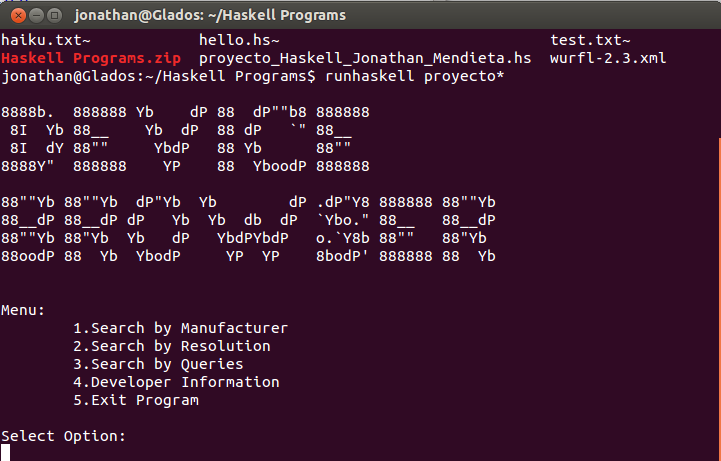
\includegraphics[scale=0.4]{screens/haskell1.png}
\end{center}
Si el usuario ingresa la opcion 1, entonces el programa presentara en una lista todos los manufacturadores de los dispositivos (brand name).\\
\begin{center}
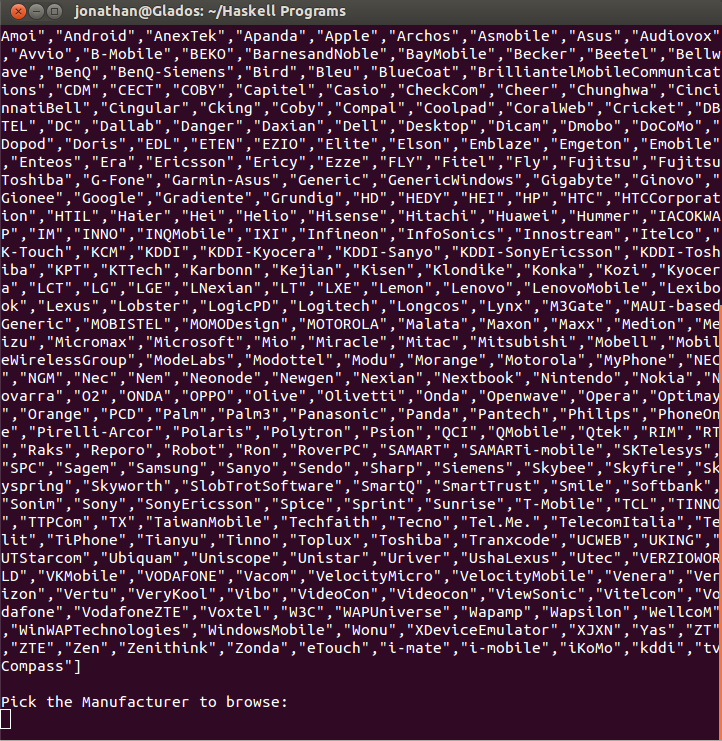
\includegraphics[scale=0.4]{screens/haskell2.png}
\end{center}
Como ejemplo elegi al manufacturador "Nokia", a continuación se mostrará los dispositivos de tal manufacturador.
\begin{center}
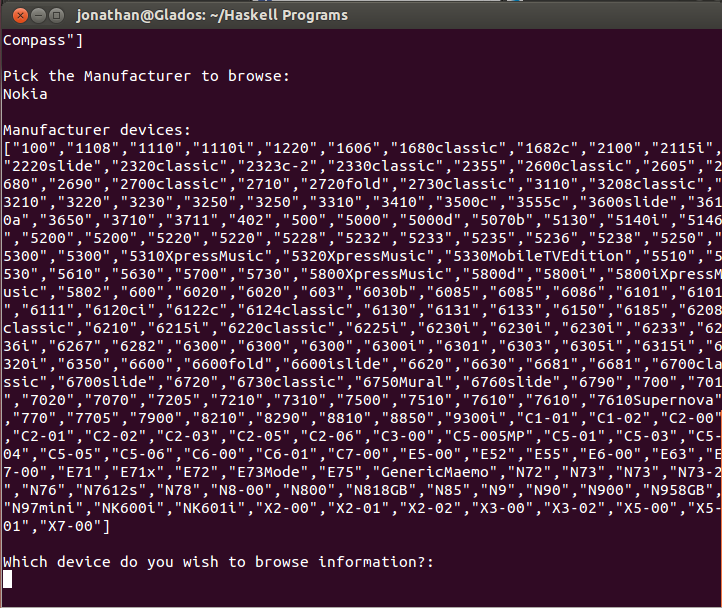
\includegraphics[scale=0.4]{screens/haskell3.png}
\end{center}
El programa mostrará la información del dispositivo a elegir, como ejemplo se eligió el modelo 6620.
\begin{center}
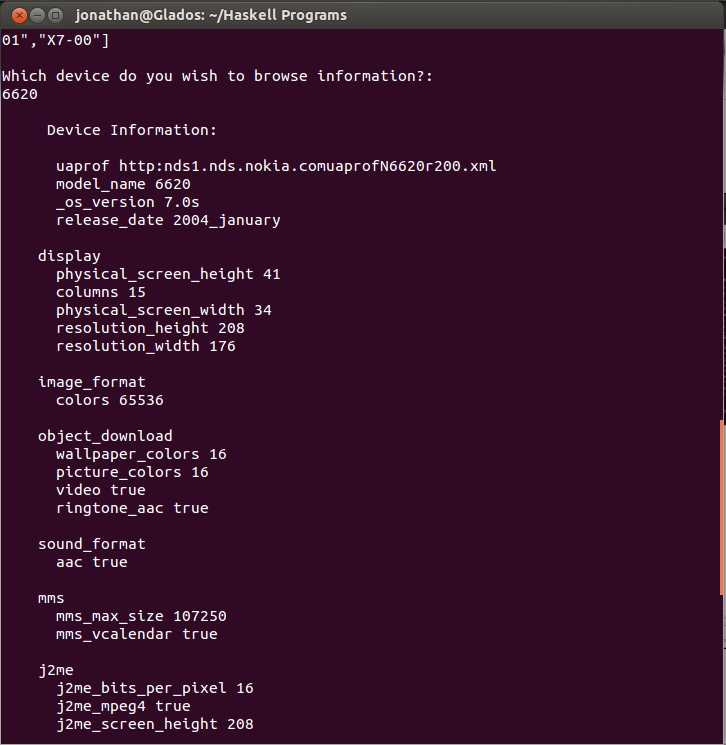
\includegraphics[scale=0.4]{screens/haskell4.png}
\end{center}
Ahora se muestra la opcion 2, en donde el programa pedirá al usuario que ingrese el manufacturador de la lista.
\begin{center}
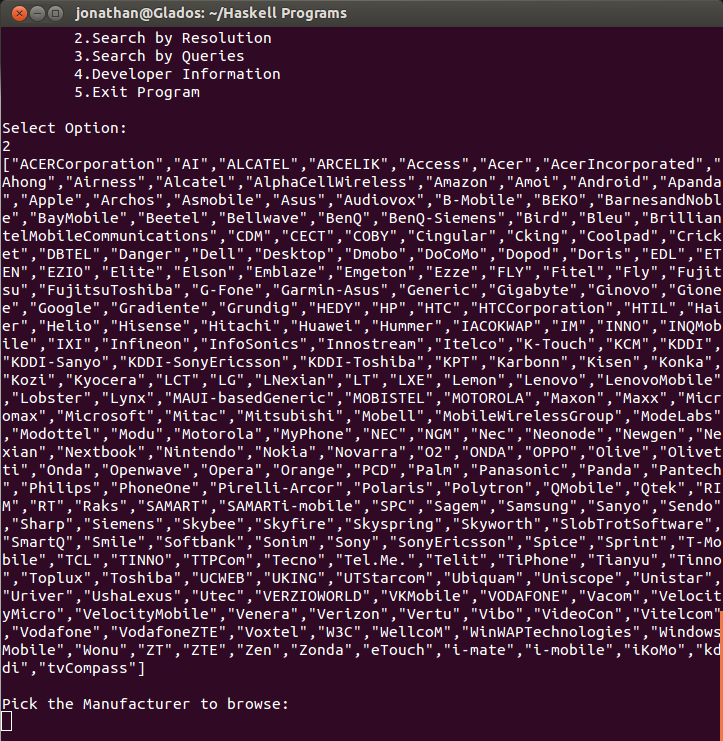
\includegraphics[scale=0.4]{screens/haskell5.png}
\end{center}
Nuevamente se eligió Nokia, ahora el programa se encargará de mostrarnos las resoluciones disponibles de sus dispositivos.
\begin{center}
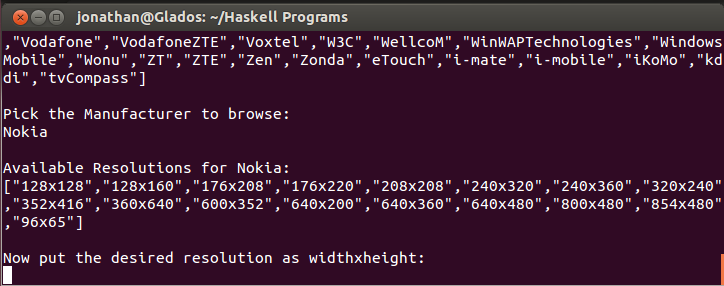
\includegraphics[scale=0.4]{screens/haskell6.png}
\end{center}
Y como proceso final, el programa mostrará los dispositivos que contienen tal resolución en una lista.
\begin{center}
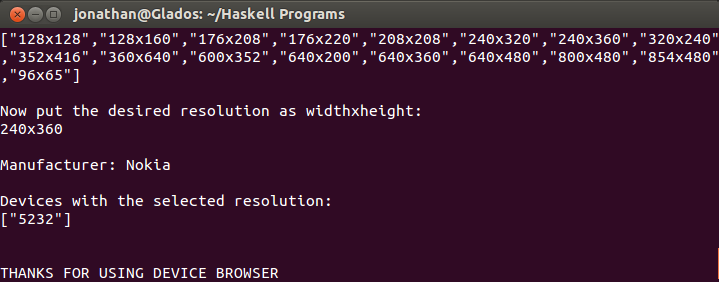
\includegraphics[scale=0.4]{screens/haskell7.png}
\end{center}
Bueno, ahora se mostrará la opcion 3 de mostrar el número y nombre de dispositivos que cumplen con los queries: brand\_name Nokia y  jpg true.
\begin{center}
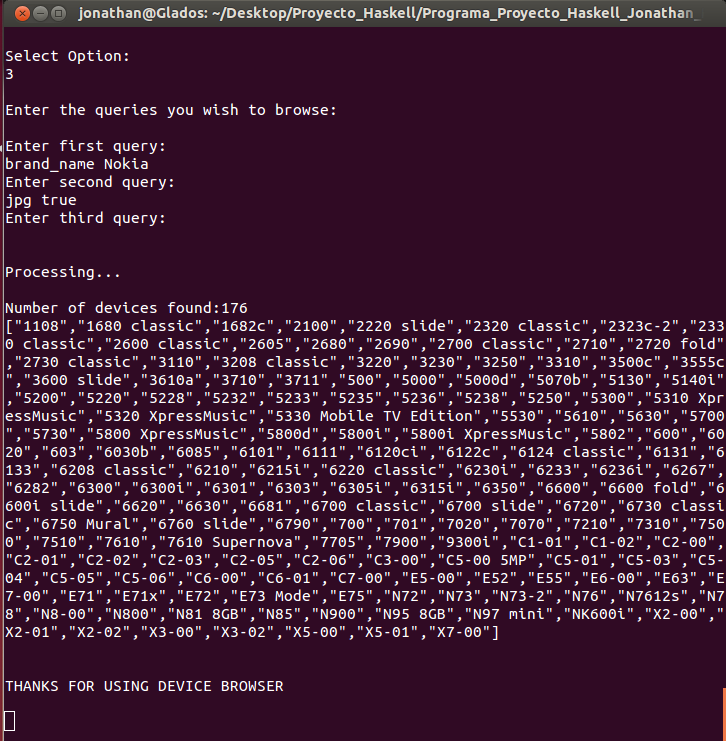
\includegraphics[scale=0.4]{screens/haskell8.png}
\end{center}
Como ultima opcion se mostrará el nombre del desarrollador del programa.
\begin{center}
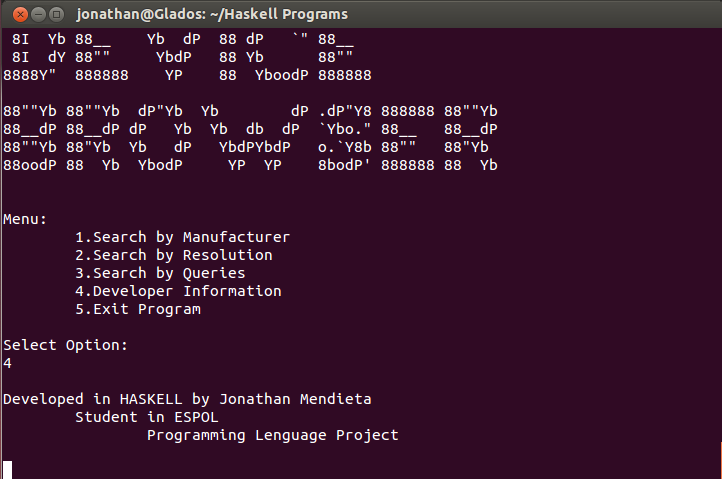
\includegraphics[scale=0.4]{screens/haskell9.png}
\end{center}
\section{FUNCIONES:}
Las funciones usadas en haskell para que esto sea posible:\\\\
--spliterInicial : Funcion para separar los devices de la cabezera principal\\
spliterInicial :: [Char] - [[Char]]\\\\
--getNames : Funcion que separa cada nombre y modelo de device en una lista\\
getNames :: [[Char]] - [([Char],[Char])]\\\\
--searchDevicesforGeneric : Funcion que obtiene devices con modelo y manufacturador\\
searchDevicesforGeneric :: [[Char]] - [[Char]]\\\\
--cleanContent : Funcion que limpia el contenido del xml como lo son los caracteres especiales\\
cleanContent :: [[Char]] - [[Char]]\\\\
--groupDevicebyManufacturer : Funcion que busca los devices por manufacturador y los bota en una lista\\
groupDevicebyManufacturer :: [Char] - [([Char],[Char])] - [[Char]]\\\\
--groupManufacturer : Funcion que bota los Manufacturadores ordenados y sin repeticion\\
groupManufacturer :: [([Char],[Char])] - [[Char]]\\\\
--deviceInformation : Funcion bota en un string la informacion del dispositivo\\
deviceInformation :: [Char] - [(([Char],[Char]),[Char])] - [Char]\\\\
--groupDevicebyResolution : Funcion que valida devices con resoluciones anchoxalto\\
groupDevicebyResolution :: [(([Char],[Char]),[Char])] - [[Char]]\\\\
--groupDevicewithResolution : Funcion que junta cada device con su respectiva resolucion widthxheight\\
groupDevicewithResolution :: [[Char]] - [([Char],[Char],[Char])]\\\\
--manufacturerwithResolution : Funcion que imprime los manufacturadores con resolucion habilitada\\
manufacturerwithResolution :: [([Char],[Char],[Char])] - [[Char]]\\\\
--devicewithResolution : Funcion que imprime las resoluciones por device\\
devicewithResolution :: [Char] - [([Char],[Char],[Char])] - [[Char]]\\\\
--deviceByResolution : Funcion que bota en una lista los dispositivos con la resolucion requerida\\
deviceByResolution :: [Char] - [Char] - [([Char],[Char],[Char])] - [[Char]]\\\\
--searchbyQuery : Funcion que busca dispositivos por los queries proveidos y los bota en una lista\\
searchbyQuery :: [Char] - [Char] - [Char] - [[Char]] - [[Char]]\\\\
--printDevicesbyQuery : Funcion que imprime los dispositivos que cumplen con los queries\\
printDevicesbyQuery :: [[Char]] - [[Char]]\\\\
\end{document}